\chapter{绪论}
% 解释:RISC-V、开源处理器、高性能、虚拟化、虚拟化扩展
% 提及:云和数据中心领域是热的,在工业界有人不断尝试,是值得做的。
% 尽管该项目可能无法实现、但是需要去尝试、合并到工业界中。
% 以未来为切入点,画大饼。
% 历史片段

% 2018年11月8日,在网信办、中科院等多个国家部委支持和指导下,
% RISC-V中国联盟于浙江乌镇举行的第五届互联网大会上正式宣布成立。
% 从成立到现在的5年见,可以看见国内RISC-V相关产业在快速的发展。
% RISC-V是一个基于精简指令集原则的指令集架构,与x86、ARM架构是对应的关系。
% 首先,RISC-V与其他指令集最大的不同点在与开源性,即不需要收取高额的版权费,
% 相对的,x86和ARM指令集知识产权的公司均为国外公司,不利于我国实现关键芯片的自主可控。
% 因此,开源意味着自由、安全及可控。
% 其次,RISC-V还具有简洁、模块化的特点,
% 意味着轻量化、低功耗、小体积,因此非常适用于移动设备,以及在多场景的灵活适应性。
% 正是具有以上特点,在计算机体系结构领域,RISC-V受到了学术界和工业界的广泛瞩目。
% 短短六年,中国目前有300家以上公司在关注RISC-V或以RISC-V指令集进行开发。
% 从嵌入式到AI服务器,各种类别的RISC-V处理器核百花齐放。
% 我们有理由相信,未来RISC-V将在中国的芯片领域有更大的应用空间和市场份额。

% 中科院计算所研究员孙凝晖院士如此说道:“
% 开源模式不仅仅是一种商业模式,也是一种生态构建方法,是一种复杂系统开发方法。
% 更蕴含着一种精神。开源不仅仅公开源代码,更重要的是协作开发流程的建立与社区治理机制的建设。”

% 和中国知网上收录的关于RISC-V的文章在2018到2023年的平均增长比例达到了17.21\%和17.37\%

% RISC-V重要性,RISC-V是什么
% 虚拟化技术的重要性,什么是虚拟化技术
% RISC-V也在不断迈向虚拟化技术,这是十分必要的一件事
% 最后说出我们的工作内容,在这里不用说调试的问题

\section{课题研究背景及研究目的和意义}
2018年11月8日,在网信办、中科院等多个国家部委支持和指导下,
RISC-V中国联盟于浙江乌镇举行的第五届互联网大会上正式宣布成立。
代表着RISC-V在我国受到各领域的广泛关注,是RISC-V在国内快速发展的一个里程碑。
RISC-V\cite{asanovic2014instruction},
是近年来计算机体系结构研究催生出的一种新型指令集架构(Instruction Set Architecture,ISA)。
它凭借其开源、简洁、模块化的特性,受到了学术界和工业界的广泛瞩目。
其中,开源性是RISC-V与其他指令集最大的不同点,即不需要收取高额的版权费。
相对的,x86和ARM指令集知识产权的公司均为国外公司,不利于我国实现关键芯片的自主可控。
开源意味着自由、安全及可控,因此推进RISC-V生态在国内的快速发展,
有利于使我国尽快摆脱核心芯片设计、知识产权、工艺技术等受制于人的不利局面。
同时,RISC-V还具有简洁、模块化的特点,这意味着轻量化、低功耗、小体积。
因此非常适用于移动设备,以及在多场景的灵活适应性。
从SiFive推出的面向自动驾驶的芯片\cite{sifive-automotive},
到阿里巴巴达摩院的玄铁RISC-V系列处理器\cite{xuantie}。
RISC-V在嵌入式领域中,已经逐渐进入由ARM、x86等主流计算机架构垄断的芯片市场。
然而,RISC-V并不止步于物联网领域的成功,研究者们正积极地探索着下一个RISC-V的潜在市场。

虚拟化技术,作为计算机科学领域的一项关键技术,为云计算和数据中心提供了核心的技术框架。
通过在计算机硬件上创建一个抽象层,虚拟化技术能够将单台计算机的硬件分成多个虚拟计算机。
每个虚拟机能够运行自己的操作系统,和其他虚拟机相互独立,同时又能被简单且可复现地构建、销毁。
这些优势与云计算的发展方向和对灵活IT解决方案的需求十分契合,真正改变了过去传统的基于物理机的运营模式。
随着服务器虚拟化已成为一种常见做法,许多企业已从物理现场数据中心转向虚拟化数据中心解决方案。
对于运营商而言,它能减少管理开支、停机时间,增强灾难恢复情况下的弹性,更充分利用硬件资源以提高效率和生产力。
对于用户而言,能够在需要时仅购买所需的计算资源,并随着工作负载的增长经济实惠地扩展这些资源。
随着近年来云数据中心及云服务提供商的快速发展,从初期的虚拟机与容器技术,
到新兴的函数即服务(Function as a Service, FaaS)与无服务器计算(Serverless)模式,
均展现出了强烈的市场需求和广阔的发展潜力。
这一趋势不断促进虚拟化技术的进步与创新,
处理器芯片行业的主要参与者开始在主流计算架构中引入硬件虚拟化支持以加速虚拟化软件的运行,
例如,Intel VT\cite{intel-VT2005Computer}以及ARM的VE扩展\cite{armve2018}。
如图\ref{fig:isa-vir}所示,RISC-V也希望能追上主流计算机架构的步伐,
处理云数据中心的不断增长的需求,因此RISC-V虚拟化硬件扩展的相关研究在不断的被积极推进。

\begin{figure}[htbp]
\centering
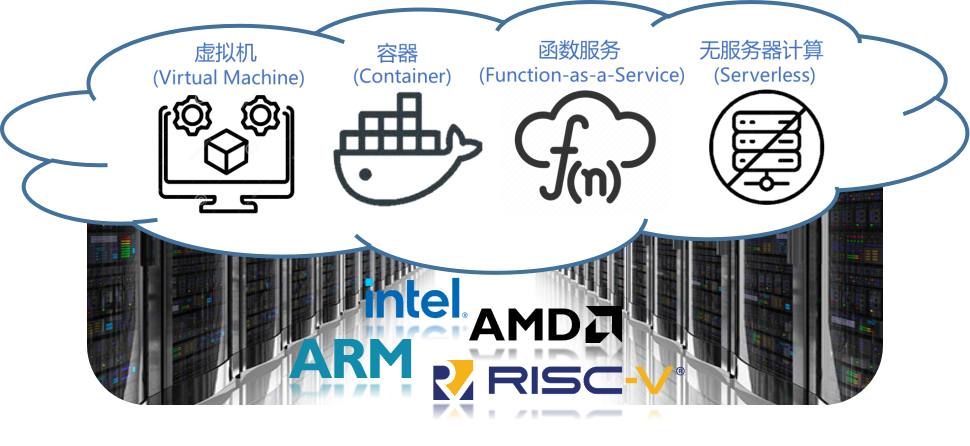
\includegraphics[scale=0.6]{virtual.png}
\caption{云数据中心在不同指令集架构的发展}
\label{fig:isa-vir}
\end{figure}

然而,关于RISC-V硬件虚拟化的研究尚处于起步阶段,研究空间依然十分巨大。
2017年,RISC-V官方提出了虚拟化扩展的概念,规定了支持虚拟化的处理器需要额外添加的特权级和指令等。
截至2021年12月,虚拟化扩展才被正式批准。
同一年,加州大学的伯克利分校迈出了虚拟化扩展硬件实现的第一步。
他们研发了Rocket Chip\cite{itco2022rocket},一个开源的RISC-V顺序流水线处理器,
在其上实现了完整的虚拟化扩展,并进行了一系列虚拟化相关的评测。
但是在真实应用场景下,处理器的情况会更为复杂,多核乱序的高性能处理器才是虚拟化服务器的主流。
然而,关高性能RISC-V的虚拟化扩展的研究尚未充分开展,
因此,本文计划瞄准高性能RISC-V处理器的虚拟化扩展实现,
计划从硬件扩展实现到管理软件适配进行全系统评测的研究。

高性能RISC-V处理器的一个典型代表便是中国科学院计算技术研究所牵头发起的“香山”项目。
作为目前国际上性能最高的开源高性能RISC-V处理器核的同时,
“香山”致力成为一个开源的工业级别处理器,并成为面向世界的体系结构创新开源平台。
计算所研究员孙凝晖院士对开源精神表示:“
开源模式不仅仅是一种商业模式,也是一种生态构建方法,是一种复杂系统开发方法。
更蕴含着一种精神。开源不仅仅公开源代码,更重要的是协作开发流程的建立与社区治理机制的建设”。
“香山”始终坚持、坚定地开源所有的设计、验证、基础工具代码,对来自社区的贡献始终表示欢迎。
因此,十分适合用于高性能RISC-V处理器的虚拟化扩展研究。

\section{国内外研究现状}
在RISC-V虚拟化拓展规范的仍处于草案阶段时,
一些主流虚拟机管理程序和模拟器就已经随着拓展的技术规范的更新进行适配,
例如Xvisor\cite{pdp2015xvisor}、KVM\cite{kvm:H-ext}、
QEMU\cite{qemu-riscv:H-ext}和Spike\cite{github:spike}等。
然而,关于虚拟化扩展的硬件实现,仅从拓展的0.6.1版本发布后才陆续出现。

虚拟化扩展的硬件实现工作最早开展在Rocket Chip\cite{itco2022rocket}中,这是加州大学伯克利分校开发的顺序单发射流水线处理器。
此外,该工作还在处理器中移植了Bao,一种轻量级的虚拟机管理系统\cite{ng-res2020bao},并且进行了一些简易的虚拟化性能评测。
2023年,一个六级流水的乱序单发射开源处理器核心CVA6\cite{tvlsi2023cva6}也实现了虚拟化扩展。
该工作不仅进行了关于两阶段地址转化技术的微架构探索,还对性能、功耗、面积等物理设计进行了一系列优化。

在商业界,StarFive发布了Dubhe系列,这是首款支持虚拟化的商业级RISC-V处理器IP核。
此外,SiFive的P600系列处理器也支持虚拟化扩展。
其他支持虚拟化扩展的处理器包括InCore Semiconductors的Chromite处理器和IIT Madras发布的Shakti处理器。
在国内,进迭时空SpcemiT也发布了实现虚拟化扩展和IOMMU的X100处理器。
这些处理器提供了硬件级别的支持,使得虚拟化技术在RISC-V体系结构中得到了广泛应用。

此外,RISC-V虚拟化扩展也常常作为可行计算的研究基础,通过虚拟化手段进行可行计算执行环境的隔离。
目前,RISC-V应用程序处理器可信执行环境的技术委员会(Application-Processor Trusted Execution Environment,AP-TEE)
正在起草面向RISC-V平台的可行计算的规范,
讨论了对于在RISC-V平台中实现精密虚拟机所需要实现的指令集扩展和非指令集扩展,被称为CoVE\cite{sahita2023cove}。

\section{本文主要研究内容}
本文的尝试研究如图\ref{fig:level}的虚拟化系统。
首先,在底层的硬件,需要为“香山”处理器的“南湖”架构——一个用于学术研究的稳定版本,添加虚拟化扩展。
第二,在扩展的处理器中运行虚拟机管理系统。
本文选用经典的Type2虚拟机管理系统Linux-KVM\cite{kvm:H-ext},并尝试在此基础上启动虚拟机。
最后,尝试在整个软硬件系统中,使用FPGA加速仿真平台进行系统级的评测和调试。

\begin{figure}[htbp]
    \centering
    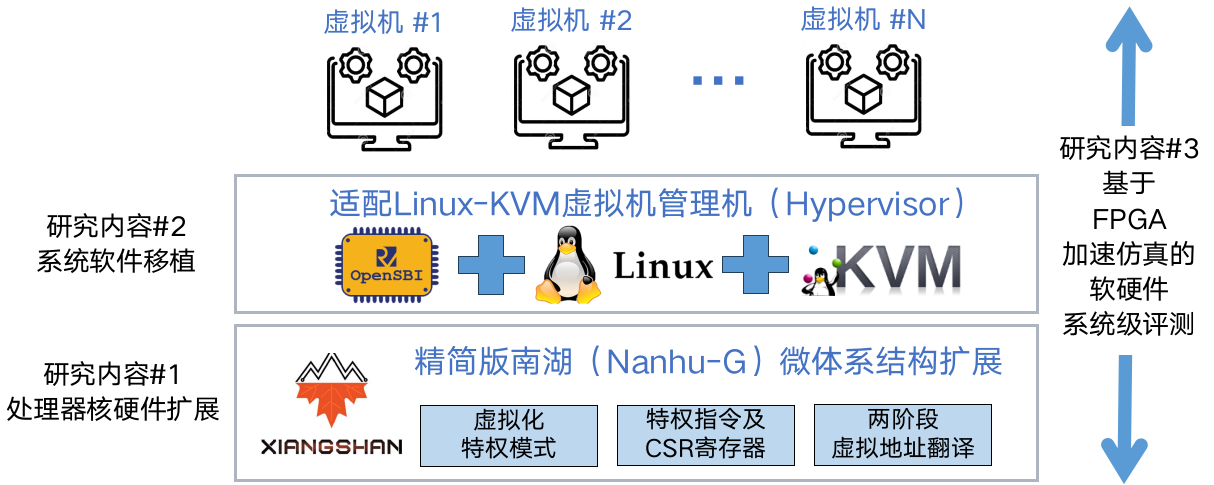
\includegraphics[scale=0.5]{level.png}
    \caption{虚拟化体系结构与本文研究内容}
    \label{fig:level}
\end{figure}

在处理器微架构方面,本文扩展了“香山”的特权管理单元和内存管理单元。
特别是虚拟内存部分,通过添加第二阶段地址翻译单元、实现了第二阶段页表翻译。
还通过复用二级页表缓存、猝发传输获取页表、压缩一级页表缓存表项等的微架构加快了翻译速度,提高了吞吐量。
在虚拟机管理软件的适配方面,本文在虚拟化扩展的“香山”中启动了Linux,并尝试使用KVM启动虚拟机。
在系统级评测中,本文完成了针对主机系统的性能评测,以及软硬件联合调试工具的创新研究。
由于在对虚拟机系统的进行性能评测时,处理器潜在的错误导致虚拟机启动失败,
因此,本文探索了通过使用体系结构检查点来跳过操作系统启动仿真程的纯软件加速手段,
和FPGA仿真加速平台联合差分测试框架的调试手段。

\section{全文章节安排}
本文由六个章节组成。
第一章作为绪论,在简要介绍本文的研究背景和动机的同时,也提出了本文的研究内容。
第二章介绍技术背景和研究动机,
一方面介绍在本文中所使用的所有专业术语和技术名词,主要包括RISC-V虚拟化扩展,“香山”内存管理单元微架构等。
另一方面也对该方向的相关研究工作进行总结,并简要地将其与本文工作进行对比。
第三章详细叙述为了实现虚拟化扩展的功能,需要对“香山”微架构进行的扩展,包括特权控制单元和内存管理单元。
重点介绍了本文权衡利弊后,所设计的能够提高吞吐、加快速度的微架构算法。
第四章介绍虚拟机管理系统的适配和启动,以及在主机系统的下的相关性能评测。
也会叙述在启动过程中遇到的错误,以及如何使用FPGA加速仿真平台解决出现的问题。
第五章叙述了在虚拟化扩展后的“香山”中尝试启动虚拟机,以及对各种软硬件联合调试方法的探索。
最后一部分作为结论,简要地总结了本文的所有工作成果。